\section{Langkah-Langkah Percobaan}
\begin{enumerate}
    \item Reset konfigurasi router dan masuk winbox.
    
    \item Konfigurasi Konfigurasi DHCP Client pada Router A (Ether 1). Sambungkan kabel internet ke ether1 pada Router A, kemudian lakukan konfigurasi DHCP Client. Akses menu IP > DHCP Client. Klik ikon "+" untuk menambah entri baru. Pilih "ether1" sebagai Interface. Klik "Apply" dan pastikan status koneksi menunjukkan "bound".
    
    \begin{center}
        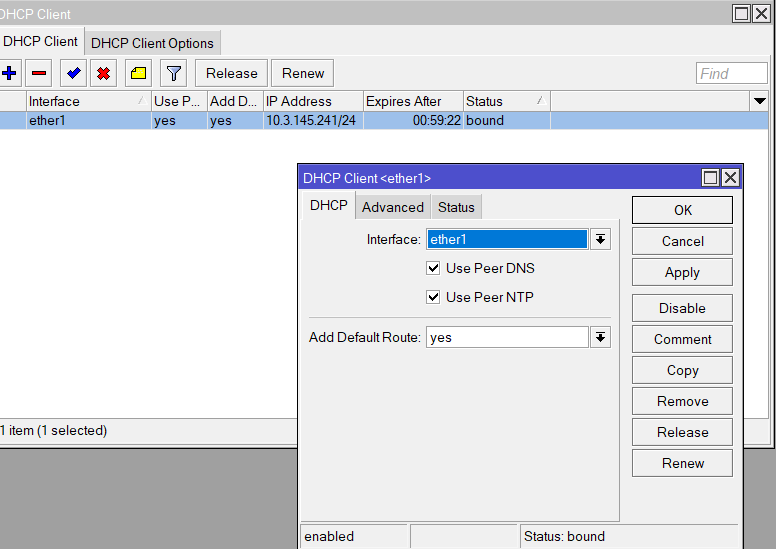
\includegraphics[scale=0.5]{P1/img/1.png}
    \end{center}
    \item Tambahkan alamat IP pada ether7 untuk konektivitas dengan Switch. Navigasikan ke menu IP > Addresses. Klik ikon "+" untuk menambahkan alamat IP. Masukkan Address: 192.168.10.1/24. Pilih Interface: "ether7". Klik "Apply" kemudian "OK".
    \begin{center}
        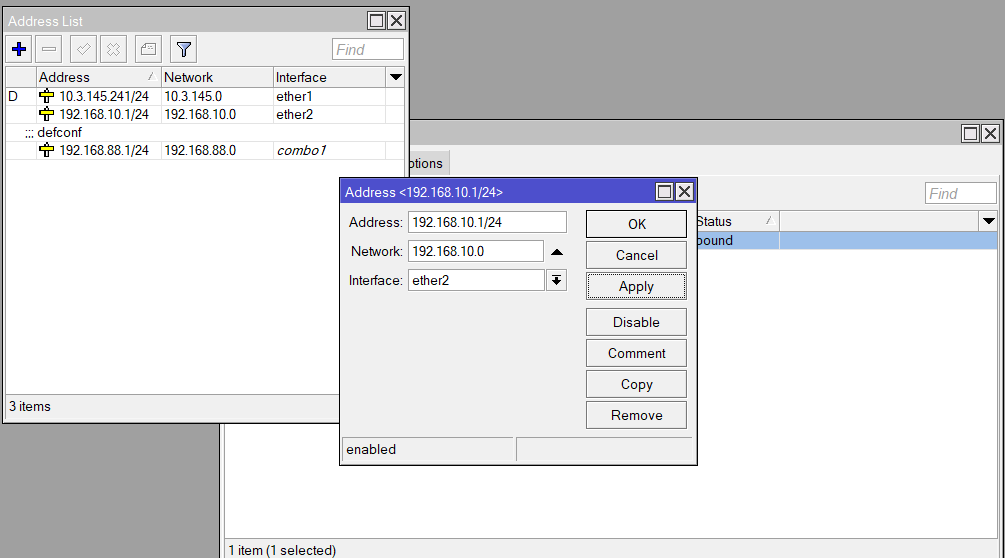
\includegraphics[scale=0.5]{P1/img/2.png}
    \end{center}
    \item Konfigurasi DHCP Server untuk secara otomatis mendistribusikan alamat IP kepada perangkat klien yang terhubung.
    \begin{itemize}
        \item Akses menu IP > DHCP Server.

        \item Klik tombol "DHCP Setup".

        \item Pada jendela "DHCP Server Interface":
        Pilih interface yang akan mendistribusikan IP address ke klien. Contoh: "ether7" (sesuai koneksi ke Switch/Client). Klik "Next".

        \item Pada jendela "DHCP Address Space":
        Verifikasi network address yang akan digunakan (contoh: 192.168.10.0/24). Klik "Next".

        \item Pada jendela "Gateway for DHCP Network":
        Verifikasi gateway yang akan diberikan kepada klien (contoh: 192.168.10.1). Klik "Next".

        \item Pada jendela "Addresses to Give Out":
        Tentukan rentang alamat IP yang akan didistribusikan (contoh: 192.168.10.2-192.168.10.254). Klik "Next".

        \item Pada jendela "DNS Servers":
        Masukkan alamat DNS Server yang akan diberikan kepada klien (contoh: 8.8.8.8 dan 8.8.4.4). Klik "Next". (DNS akan Otomatis dapat)

        \item Pada jendela "Lease Time":
        Atur durasi waktu lease IP address (contoh: 00:10:00 untuk 10 menit). Klik "Next".
    \end{itemize}
    
    Setelah semua langkah selesai, akan muncul pesan "Setup has completed successfully". Klik "OK".
    \begin{center}
        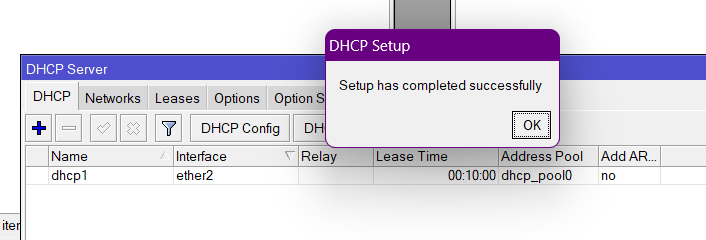
\includegraphics[scale=0.7]{P1/img/10.png}
    \end{center}
    \item Lakukan konfigurasi NAT (Network Address Translation) untuk menyediakan konektivitas internet.
    \begin{itemize}
        \item Akses menu IP > Firewall > NAT.

        \item Klik ikon "+" untuk membuat aturan baru.

        \item Pada tab "General", atur Chain: "src-nat".

        \item Pada tab "Action", atur Action: "masquerade".

        \item Klik "Apply" kemudian "OK".
    \end{itemize}
    \begin{center}
        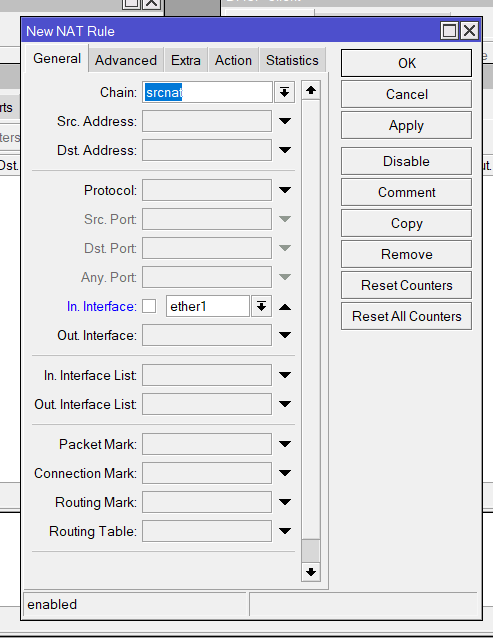
\includegraphics[scale=0.5]{P1/img/13.png}
    \end{center}
    \begin{center}
        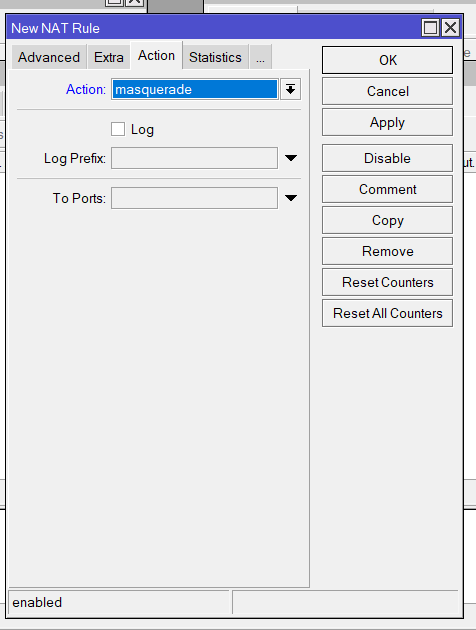
\includegraphics[scale=0.5]{P1/img/14.png}
    \end{center}
    
    Untuk test buka Terminal pada winbox dan test ping ke "ping 8.8.8.8" pastikan reply.
    \begin{center}
        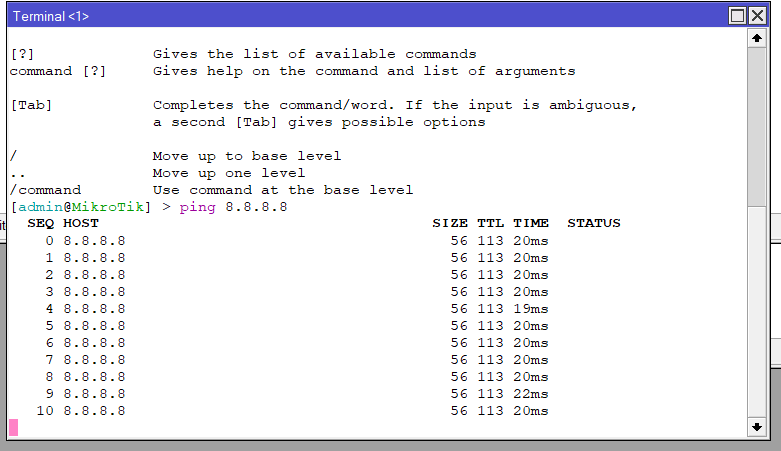
\includegraphics[scale=0.5]{P1/img/12.png}
    \end{center}

    \item Tambahkan aturan filter (Filter Rules) pada firewall.
    \begin{itemize}
        \item Akses menu IP > Firewall > Filter Rule.
        \item Klik ikon "+" untuk menambahkan aturan baru.
    \end{itemize}

    Untuk Pemblokiran ICMP (Internet Control Message Protocol):
    \begin{itemize}
        \item Pada tab "General", atur Chain: "forward".
        \item Pada tab "General", atur Protocol: "icmp".
        \item Pada tab "General", atur In. Interface: "ether7".
        \item Pada tab "Action", atur Action: "drop".
    \end{itemize}

    Untuk Pemblokiran Akses Situs Web Berdasarkan Konten (Content Blocking):
    \begin{itemize}
        \item Pada tab "General", atur Chain: "forward".
        \item Pada tab "General", atur Protocol: "tcp".
        \item Pada tab "General", atur Dst. Port: "80,443".
        \item Pada tab "General", atur In. Interface: "ether7".
        \item Pada tab "General", atur Out. Interface: "ether1".
        \item Pada tab "Advanced", atur Content: "speedtest".
        \item Pada tab "Action", atur Action: "drop".
    \end{itemize}

    \begin{center}
        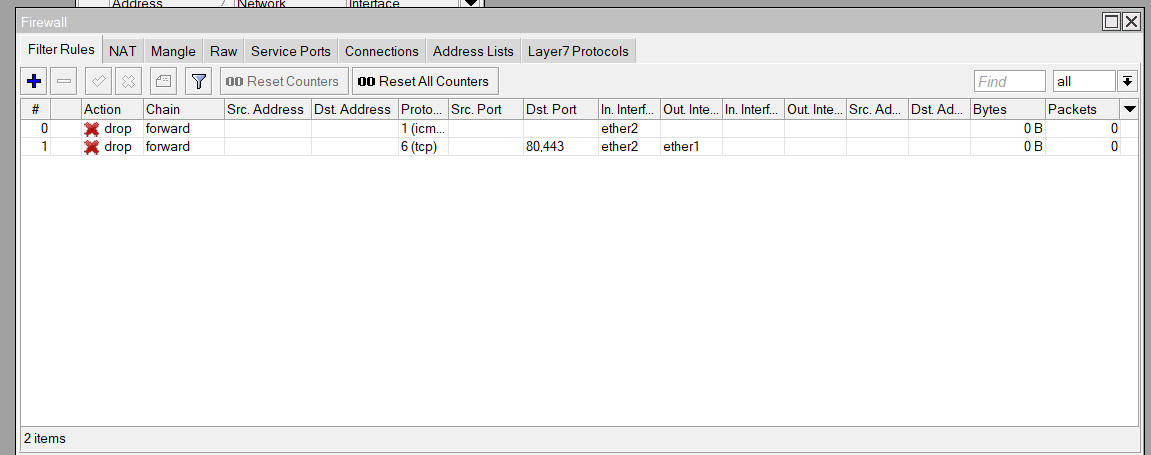
\includegraphics[scale=0.5]{P1/img/20.png}
    \end{center}

    \item Lakukan konfigurasi bridge untuk mengubah fungsi Router B menjadi hub.
    \begin{itemize}
        \item Akses menu Bridge.
        \item Klik ikon "+" untuk membuat bridge baru.
        \item Klik "Apply" kemudian "OK".
    \end{itemize}

    Selanjutnya, tambahkan port ke dalam bridge yang telah dibuat:
    \begin{itemize}
        \item Akses menu Bridge > Port.
        \item Klik ikon "+" untuk menambahkan port.
        \item Pilih interface yang terhubung ke perangkat laptop.
        \item Pilih interface yang terhubung ke Router A.
    \end{itemize}

    \item Pastikan pengaturan alamat IP pada laptop diatur secara otomatis melalui DHCP, lalu verifikasi perolehan alamat IP. Pada pengaturan sistem operasi laptop Anda (melalui Settings atau Control Panel), pastikan konfigurasi jaringan diatur ke DHCP (Automatic). Buka Command Prompt (CMD). Gunakan perintah ipconfig untuk memeriksa dan mengonfirmasi alamat IP yang telah diterima oleh laptop Anda.

    \begin{center}
        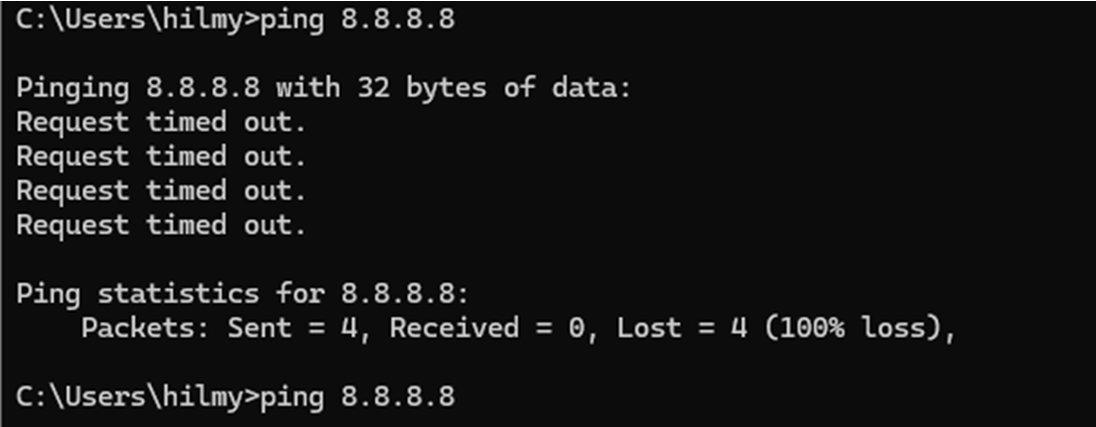
\includegraphics[scale=0.5]{P1/img/ireng1.png}
    \end{center}
    \begin{center}
        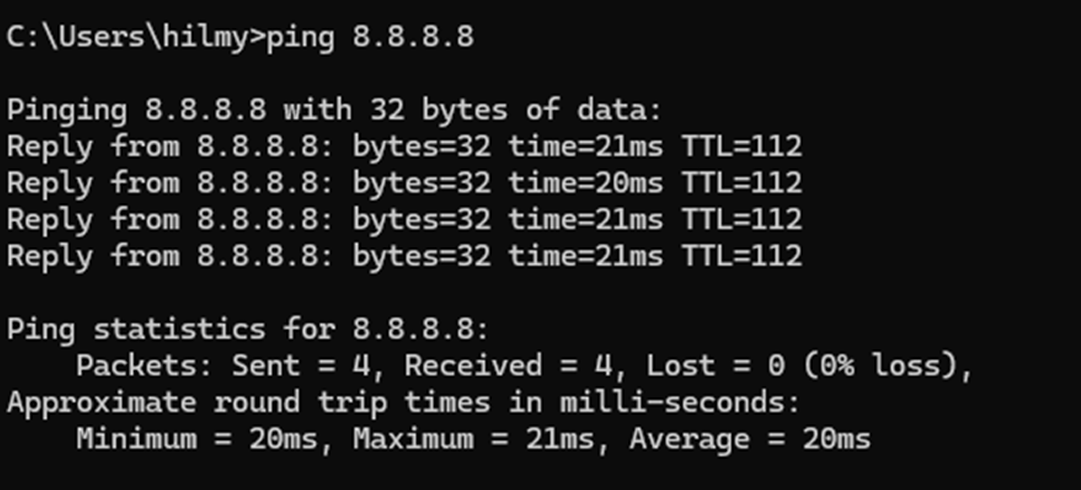
\includegraphics[scale=0.5]{P1/img/ireng2.png}
    \end{center}
    \begin{center}
        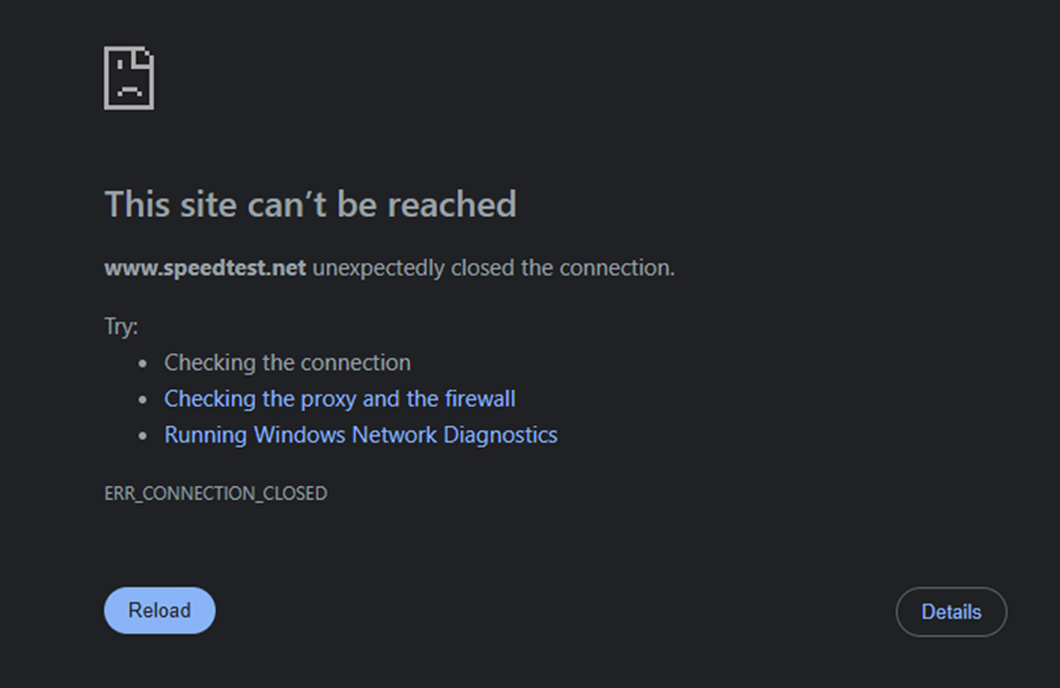
\includegraphics[scale=0.5]{P1/img/ireng3.png}
    \end{center}
    \begin{center}
        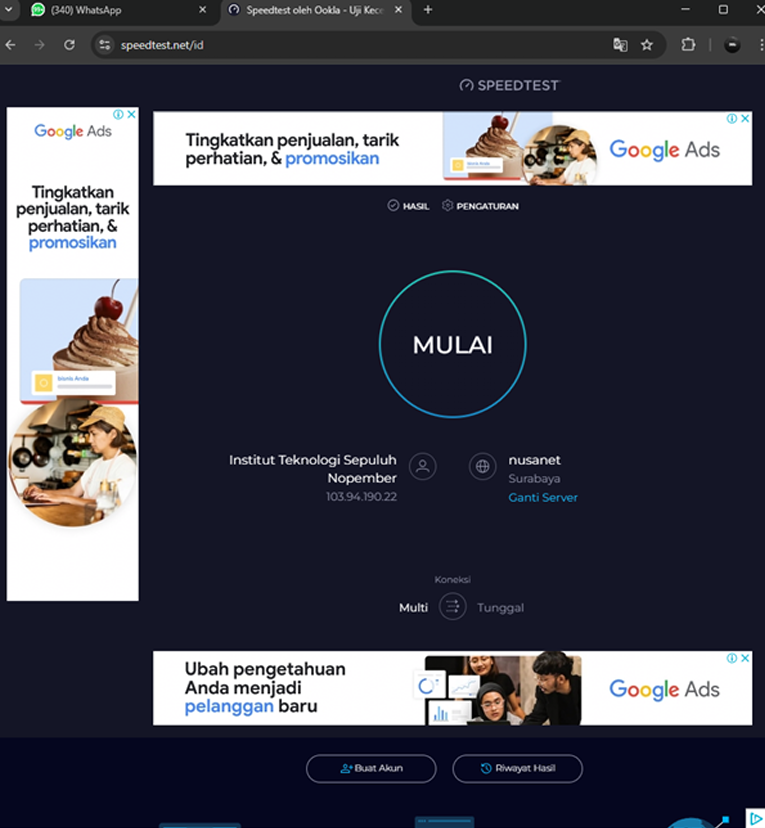
\includegraphics[scale=0.5]{P1/img/ireng4.png}
    \end{center}

\end{enumerate}
\section{Analisis Hasil Percobaan}
Secara keseluruhan, praktikum ini terlaksana dengan baik dan berhasil mencapai tujuan yang telah dirancang sebelumnya. Proses konfigurasi router dan pengelolaan jaringan yang dilakukan mampu merepresentasikan penerapan konsep teori ke dalam praktik nyata.

Pada tahap awal, konfigurasi DHCP Client pada Router A sukses menghubungkan perangkat ke jaringan ISP serta memperoleh alamat IP secara otomatis, sejalan dengan konsep DHCP yang bertujuan mempermudah pemberian alamat IP. Penambahan alamat IP pada ether7 juga telah dilakukan untuk memastikan konektivitas dengan switch berjalan dengan baik, serta mendukung penerapan teori subnetting dalam pembagian jaringan secara efisien.

Kemudian, konfigurasi DHCP Server pada router MikroTik berhasil memberikan alamat IP kepada perangkat yang terhubung, sesuai dengan prinsip DHCP yang memungkinkan distribusi IP secara otomatis dan efektif. Konfigurasi NAT juga berhasil diterapkan, memungkinkan perangkat di jaringan lokal untuk mengakses internet menggunakan satu alamat IP publik, sesuai dengan peran NAT dalam efisiensi penggunaan IP publik.

Pengujian firewall menunjukkan bahwa aturan-aturan yang ditetapkan mampu memblokir lalu lintas yang tidak diinginkan, seperti pemblokiran ICMP maupun konten tertentu di web, yang selaras dengan fungsi firewall sebagai pelindung lalu lintas jaringan. Secara keseluruhan, kegiatan ini menunjukkan pemahaman yang cukup baik terhadap teori dan implementasinya. Meskipun sempat terdapat beberapa kekeliruan kecil dalam konfigurasi, hal tersebut tidak mengganggu hasil akhir dari percobaan, yang membuktikan bahwa konsep dasar manajemen jaringan seperti DHCP, NAT, dan firewall dapat diterapkan dengan tepat.
\section{Hasil Tugas Modul}
\begin{enumerate}
    \item Buatlah topologi sederhana di Cisco Packet Tracer dengan:
    \begin{itemize}
        \item 1 Router
        \item 1 Switch
        \item 3 PC (LAN)
        \item 1 Server (Internet/Public)
    \end{itemize}
    \begin{center}
        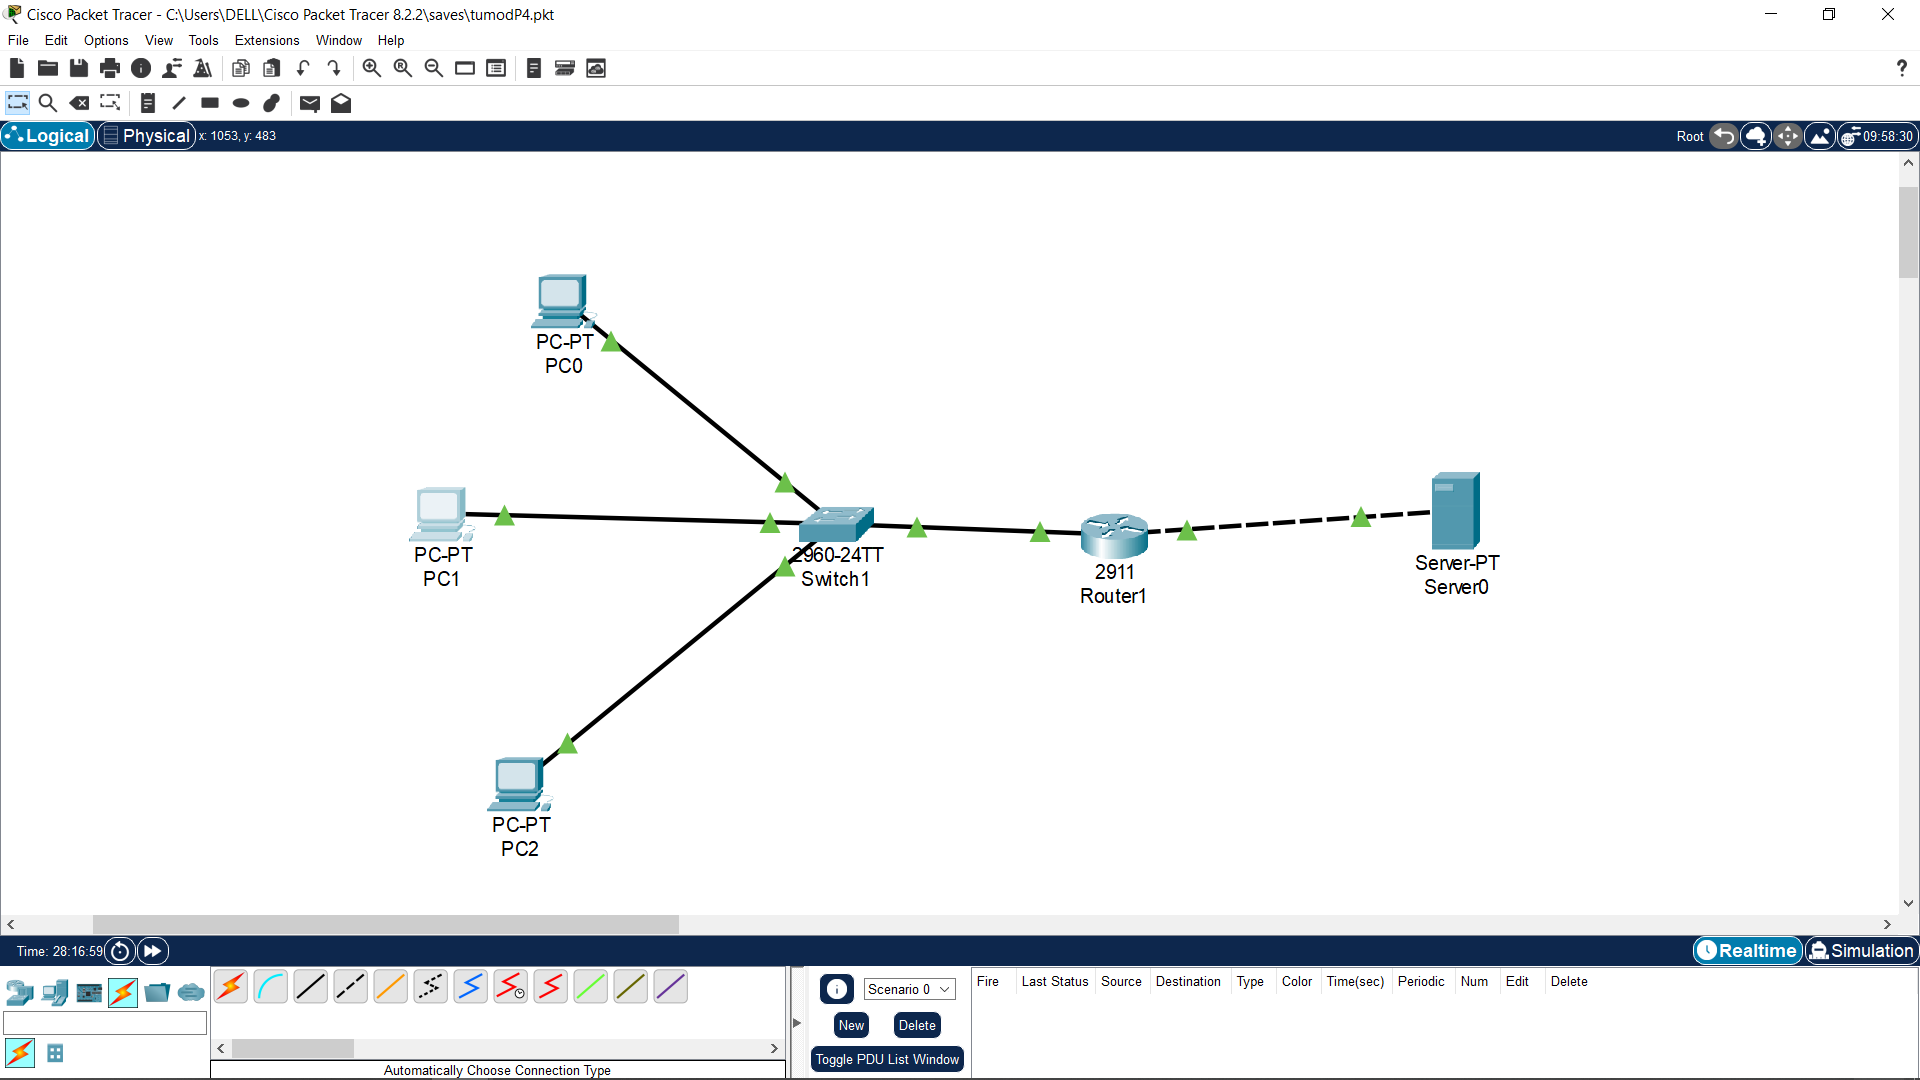
\includegraphics[scale=0.2]{P1/img/25.png}
    \end{center}

    \item Konfigurasi NAT: Buat agar semua PC bisa mengakses Server menggunakan IP publik Router.
    \begin{center}
        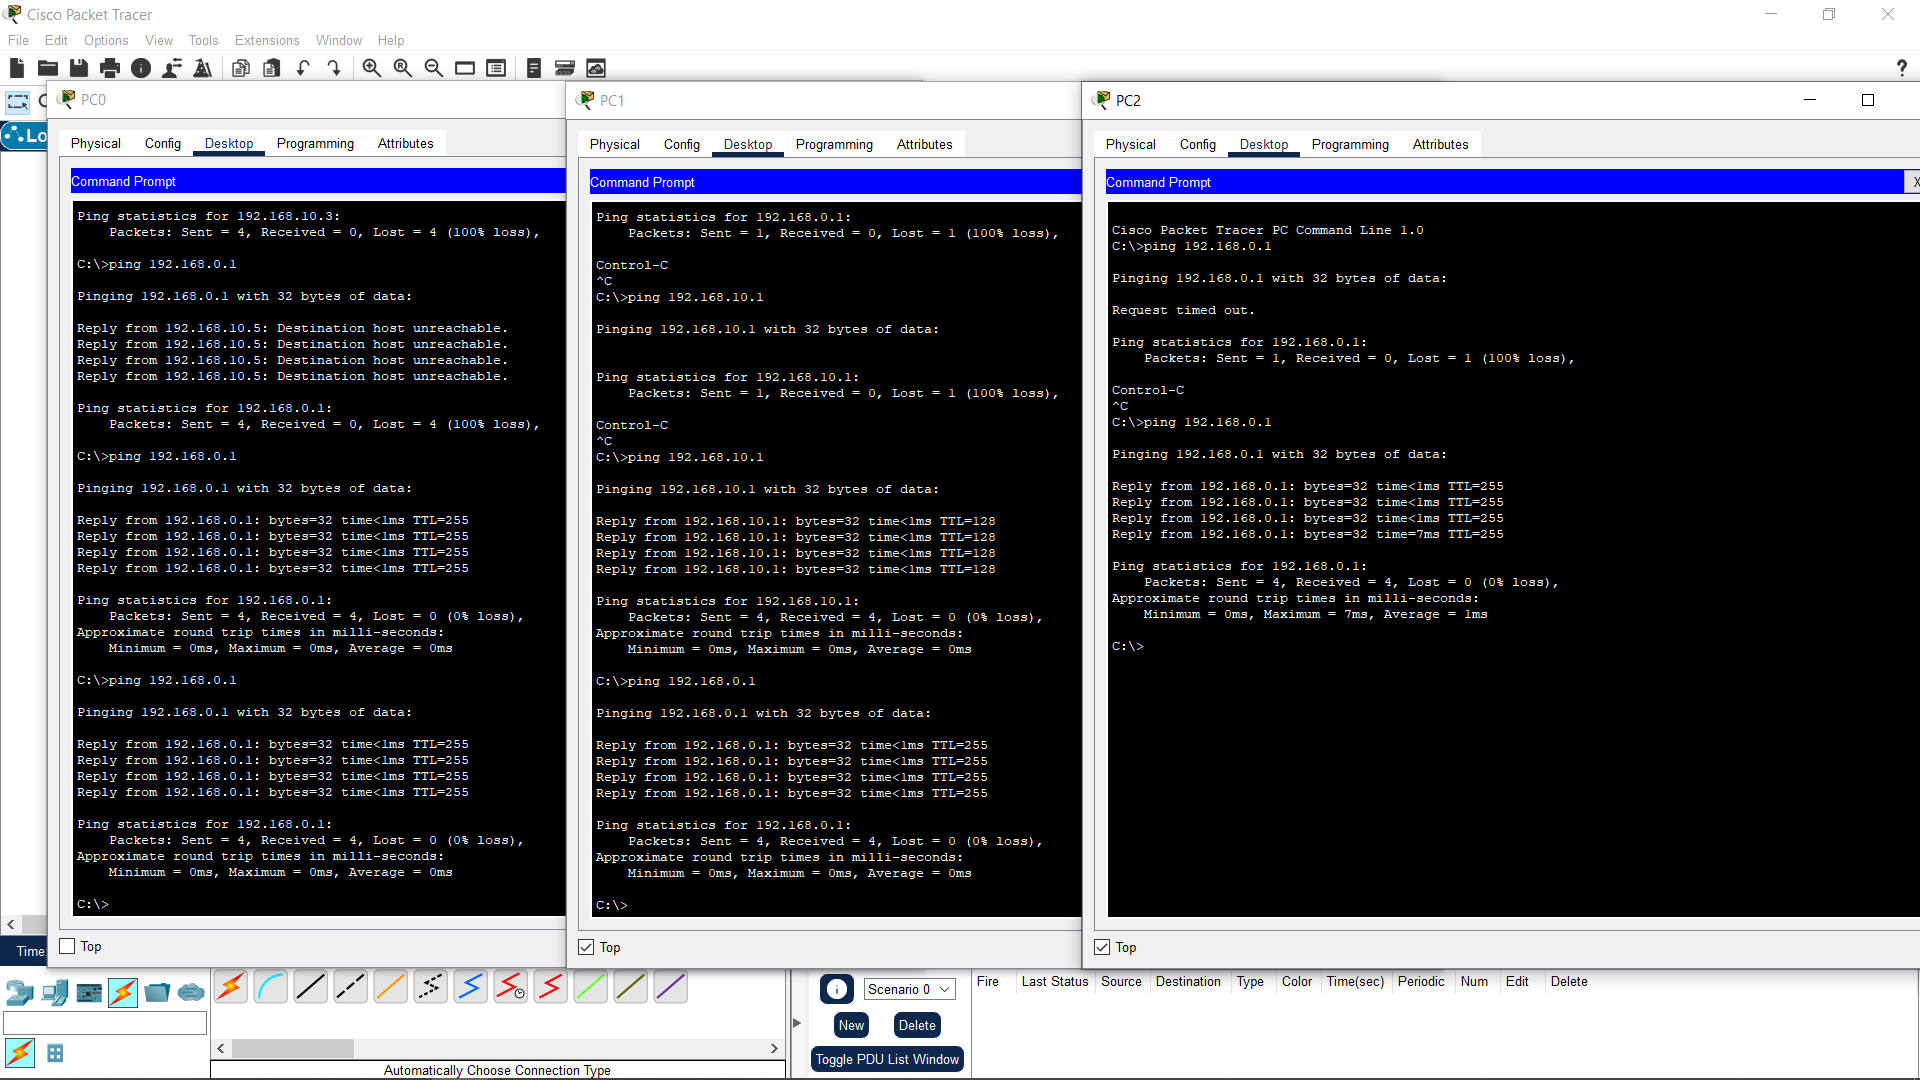
\includegraphics[scale=0.2]{P1/img/23.png}
    \end{center}

    \item Konfigurasi Firewall (ACL):
    \begin{itemize}
        \item Izinkan hanya PC1 yang dapat mengakses Server.
        \item Blokir PC1 dan PC3 dari mengakses Server.
        \item Semua PC harus tetap bisa saling terhubung di LAN.
    \end{itemize}
    \begin{center}
        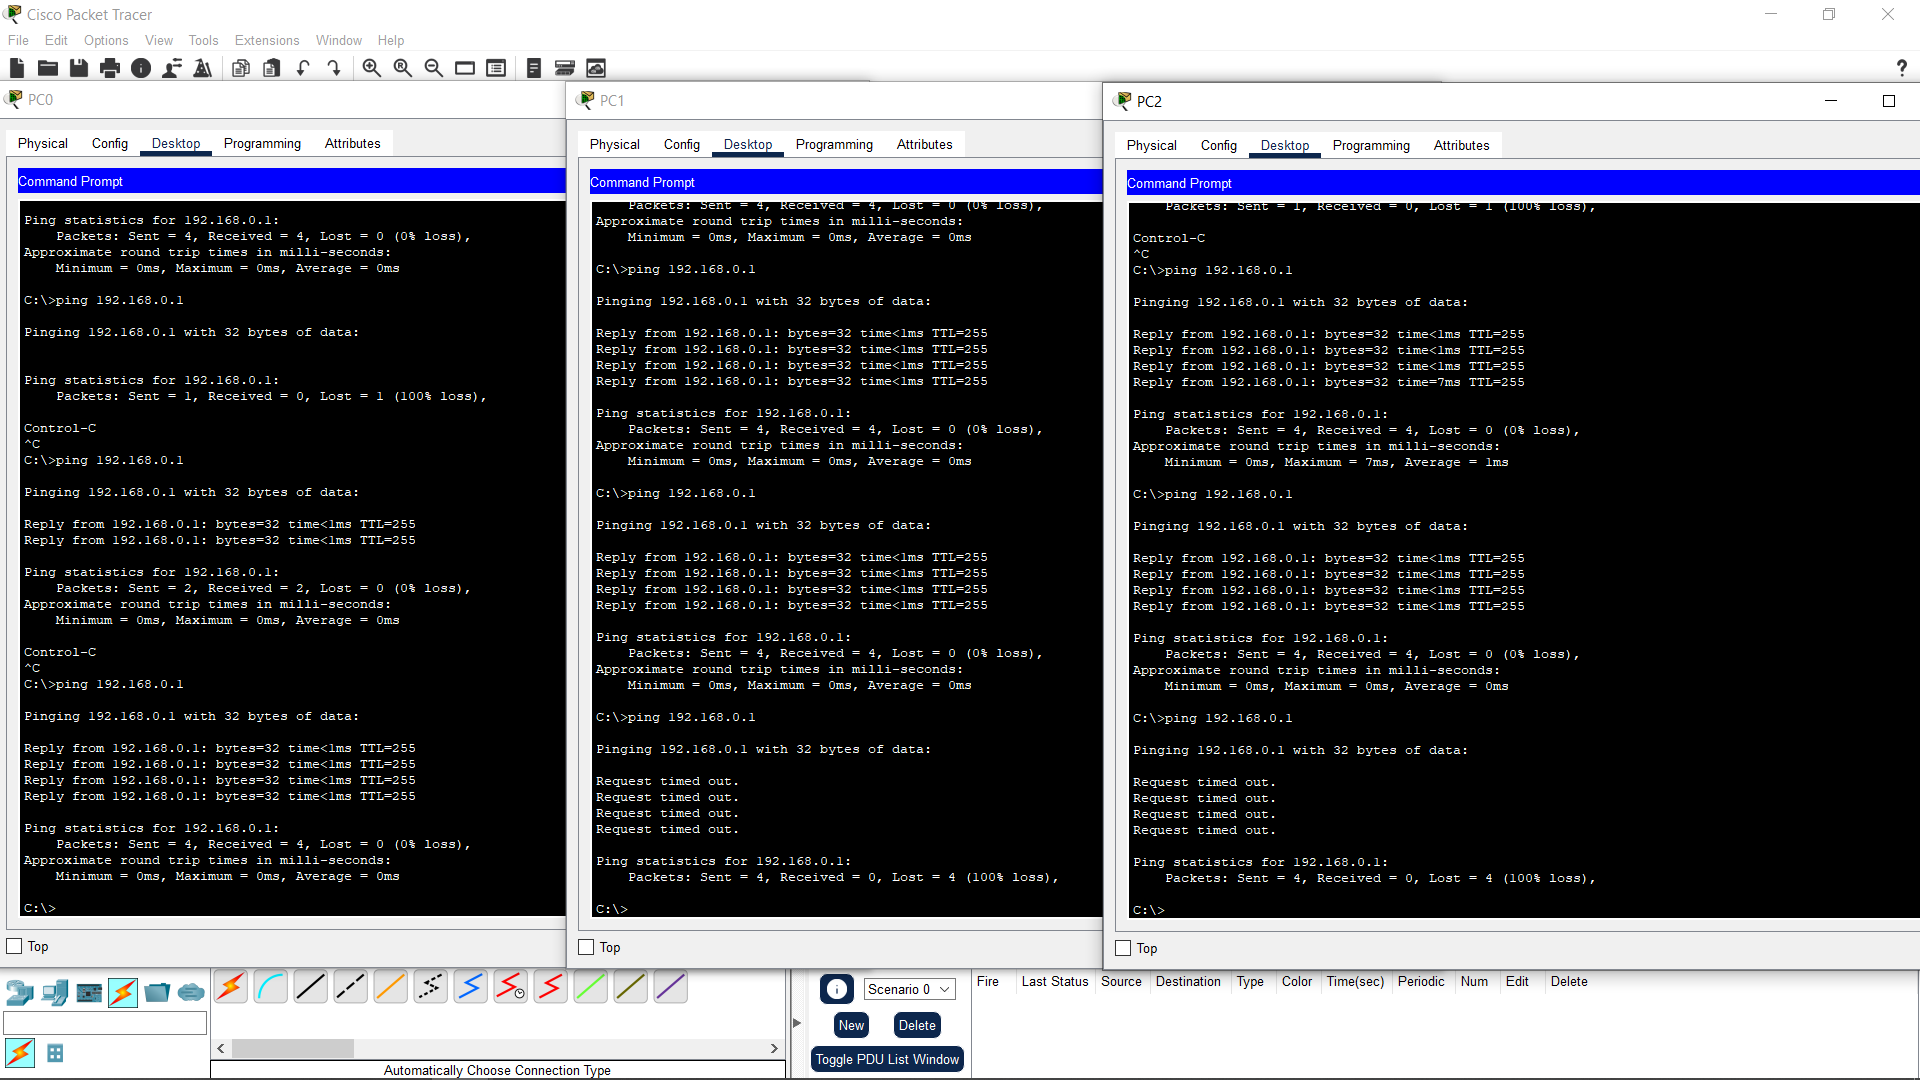
\includegraphics[scale=0.2]{P1/img/24.png}
    \end{center}
    
\end{enumerate}
\section{Kesimpulan}
Firewall dan NAT merupakan dua komponen penting dalam manajemen jaringan yang memiliki peran berbeda namun saling melengkapi. NAT (Network Address Translation) memungkinkan perangkat dalam jaringan lokal menggunakan satu alamat IP publik untuk mengakses internet, sehingga membantu menghemat penggunaan alamat IP publik yang terbatas dan meningkatkan keamanan dengan menyembunyikan struktur internal jaringan. Sementara itu, firewall berfungsi sebagai pelindung jaringan dengan mengontrol dan memfilter lalu lintas data berdasarkan aturan tertentu, guna mencegah akses yang tidak sah dan ancaman dari luar. Dengan konfigurasi yang tepat, penerapan NAT dan firewall secara bersamaan dapat meningkatkan efisiensi dan keamanan jaringan secara signifikan.
\section{Lampiran}
\subsection{Dokumentasi saat praktikum}
\begin{center}
        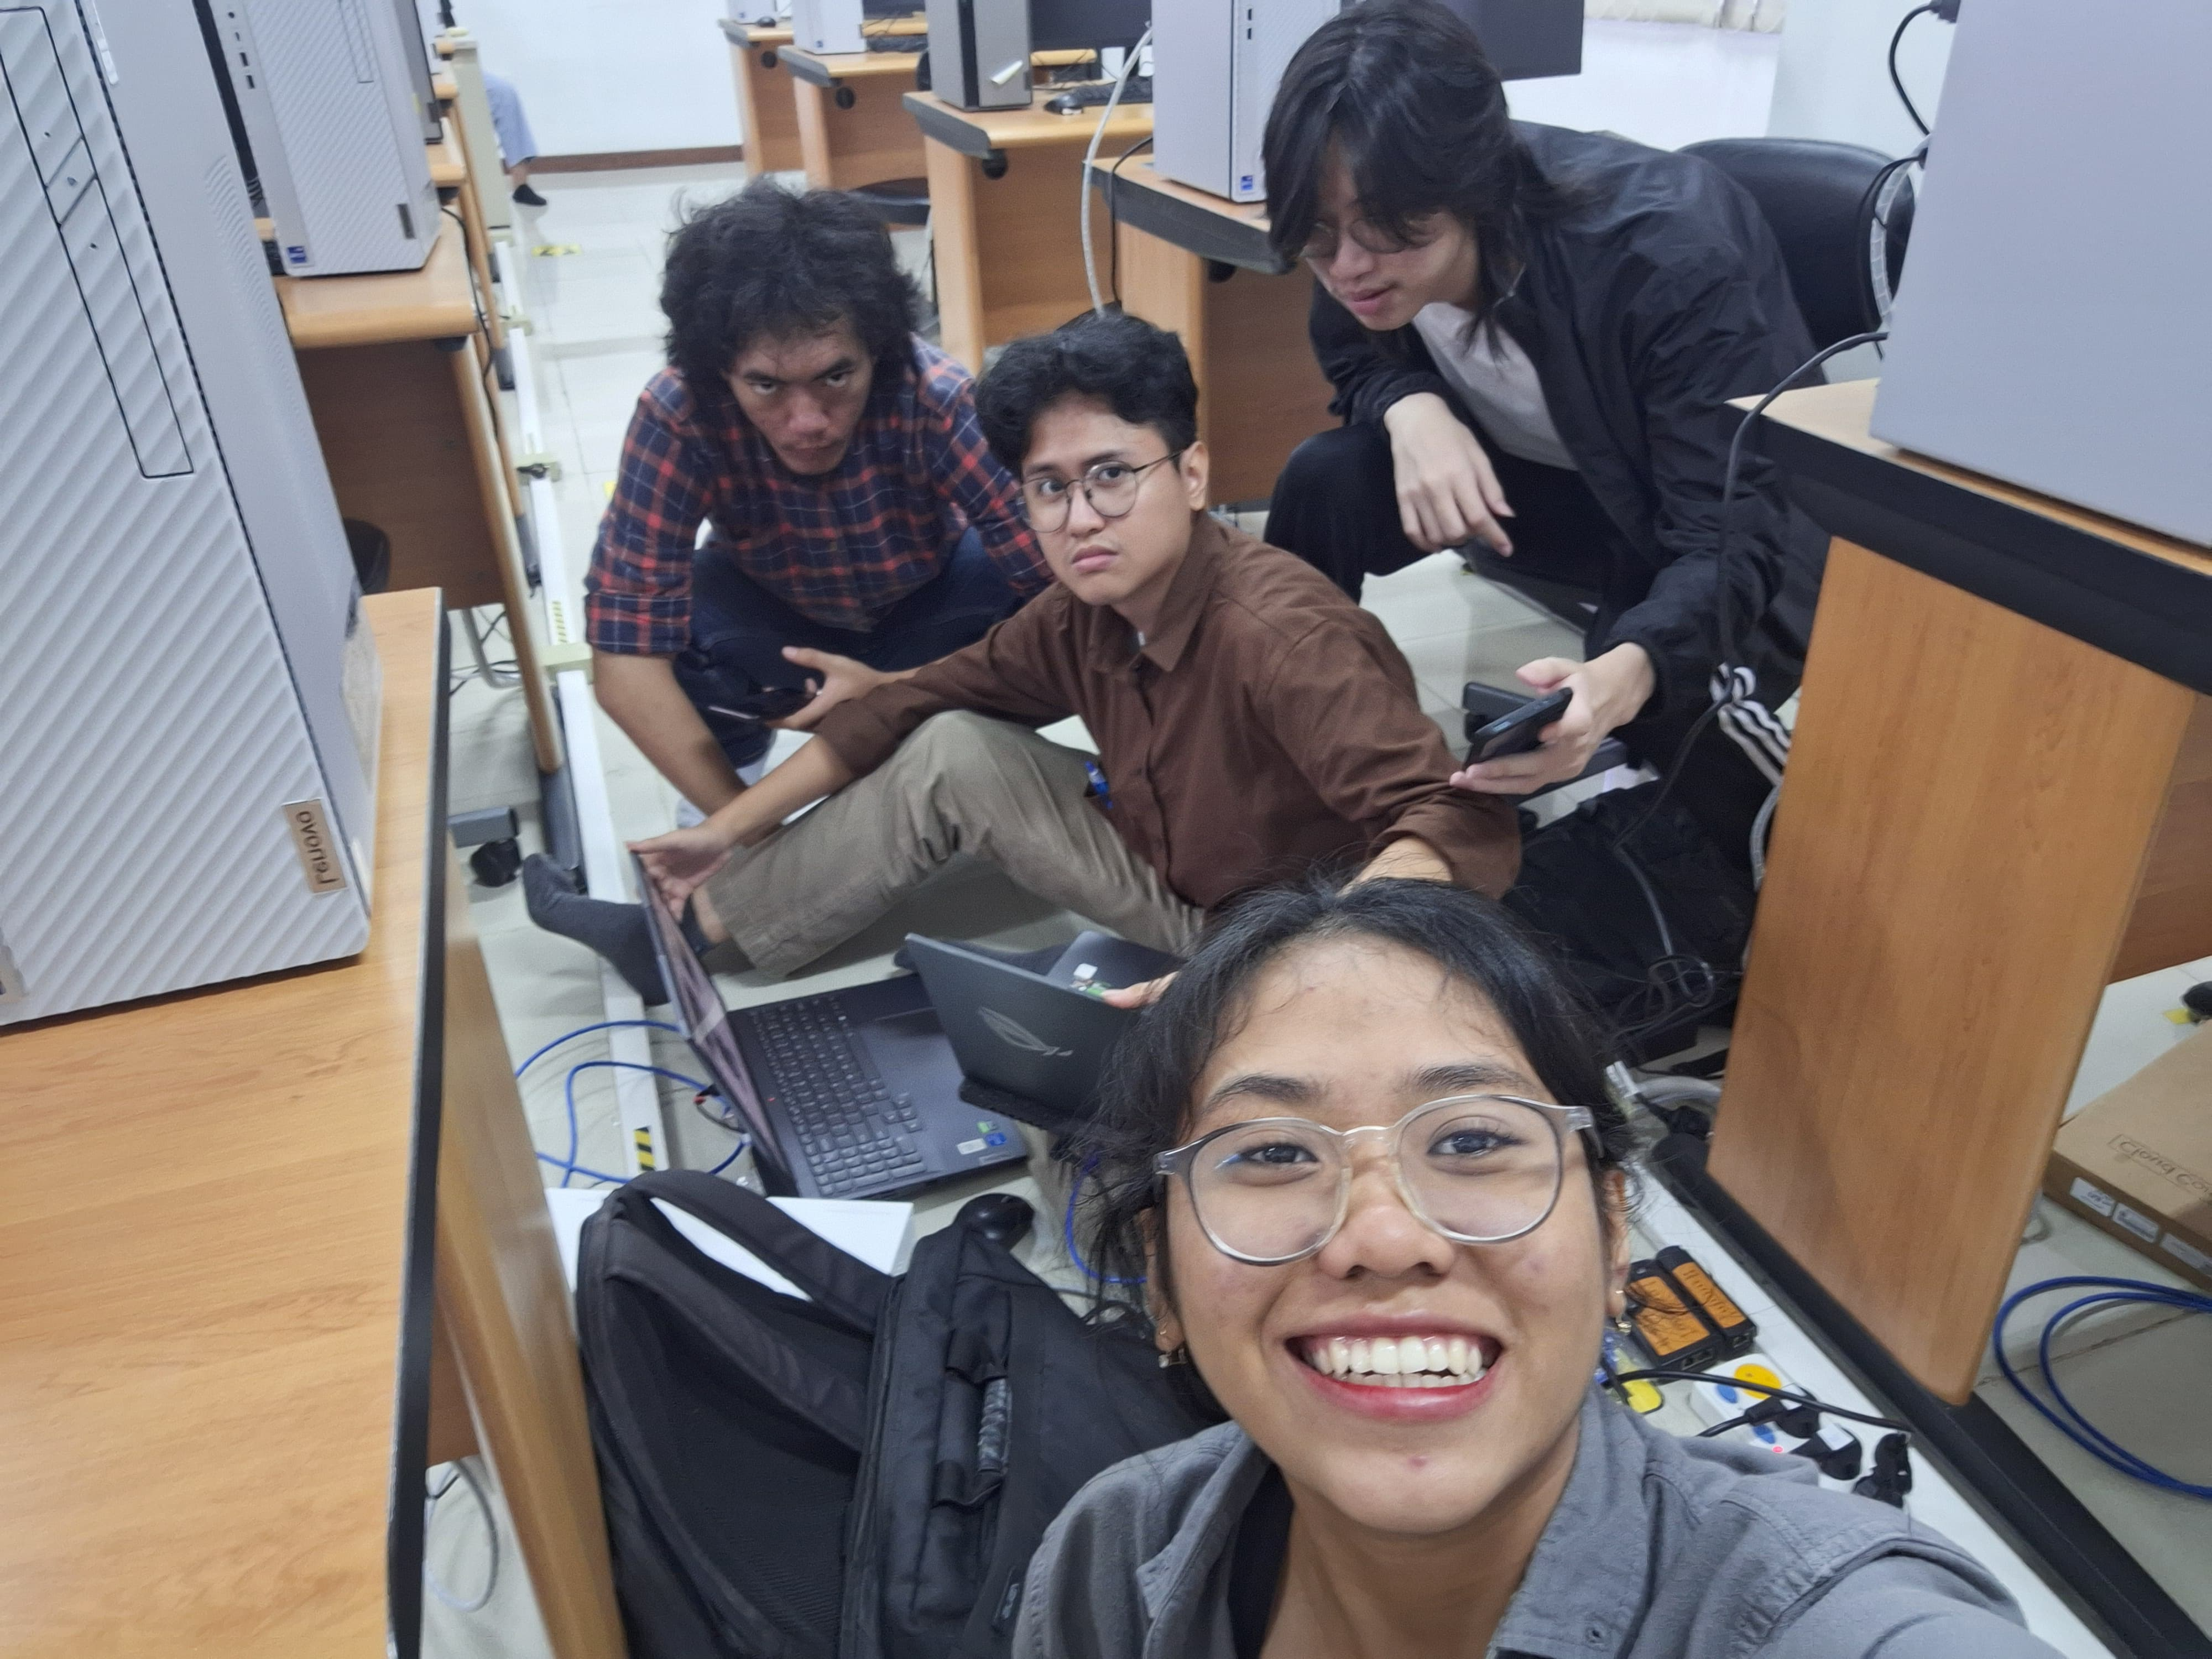
\includegraphics[scale=0.1]{P1/img/dokum.jpg}
    \end{center}